\documentclass[11pt,a4paper]{article}
\usepackage[T1]{fontenc}
\usepackage[utf8]{inputenc}
\usepackage{lmodern}
\usepackage[margin=2.5cm]{geometry}
\usepackage{amsmath,amssymb,bm}
\usepackage{booktabs}
\usepackage{upgreek}
% lightweight replacements for siunitx (the installed siunitx is incompatible with the LaTeX kernel)
\newcommand{\micro}{\upmu}\newcommand{\metre}{m}\newcommand{\kelvin}{K}
\newcommand{\micrometre}{\upmu m}\newcommand{\microkelvin}{\upmu K}
\newcommand{\SI}[2]{\ensuremath{#1\,\mathrm{#2}}}
\newcommand{\si}[1]{\ensuremath{\mathrm{#1}}}
\usepackage{graphicx}
\usepackage{tikz}
\usepackage{pgfplots}
\pgfplotsset{compat=1.17}
\usepgfplotslibrary{groupplots}
\usepackage[numbers,sort&compress]{natbib}
\usepackage[colorlinks=true,linkcolor=blue!50!black,citecolor=blue!50!black,urlcolor=blue!50!black]{hyperref}
\usepackage{caption}
\captionsetup{font=small,labelfont=bf}

\newcommand{\ket}[1]{|#1\rangle}
\newcommand{\bra}[1]{\langle #1|}
\newcommand{\gp}{\ket{g_p}}
\newcommand{\gc}{\ket{g_c}}
\newcommand{\Om}{\Omega}
\newcommand{\etaeff}{\eta_{\perp}}

\title{Radial EIT cooling of lattice-trapped $^{87}$Rb atoms in hollow-core fibres\\[2pt]
\large using higher-order guided modes: background theory, scaling trends,\\ and comparison with Raman sideband cooling}
\author{}
\date{November 2026}

\begin{document}
\maketitle

\begin{abstract}
We collect the theory needed to judge whether lattice-trapped $^{87}$Rb atoms inside a hollow-core photonic-crystal fibre (HC-PCF) can be cooled radially with electromagnetically-induced-transparency (EIT) cooling. If all beams are guided in the fundamental LP$_{01}$ mode, the dark state does not depend on the radial coordinate, so EIT cooling acts only axially. A probe beam in an LP$_{1m}$ higher-order mode, with its node on the fibre axis, together with an LP$_{01}$ coupling beam, gives a sideband coupling that is linear in the radial displacement and has no carrier. The effective radial Lamb--Dicke parameter is $\etaeff=G_{1m}x_0/a$, where $a$ is the core radius and $G_{1m}\simeq 0.46\,u_{1m}^{3/2}$ is a geometric factor that grows with mode order. In a conventional configuration, where the carrier is present, the cooling rate scales as $\etaeff^2\propto G_{1m}^2/a^2$. That is a few tens of s$^{-1}$ for a \SI{30}{\micrometre} core and LP$_{11}$. In the carrier-free node configuration, the small $\etaeff$ appears only as a probe-power penalty, which is at the nW level. The rate is then bounded by the width of the narrow EIT resonance, $\sim\nu_r/10$, i.e.\ $10^3$--$10^4\,$s$^{-1}$ for an ideal $\Lambda$ system. Very high-order modes ($m\gg1$) increase the cooling rate as $u_{1m}^3$ in the $\eta^2$-limited regime. In the node regime they mainly reduce the required power and the sensitivity to mode impurity. They also shrink the capture range ($\propto a/u_{1m}$) and add loss. Larger cores transmit more modes over a given length ($N\propto a^3/\lambda^2L$). Fibre loss turns this into a core-size trade-off through the growth of LP$_{01}$ contamination along the fibre, and the optimum mode loses about 6.5\,dB over the fibre section. For low-loss inhibited-coupling fibres the smallest core with a clean LP$_{11}$ or LP$_{12}$ remains optimal; only lossy fibres push the optimum to $a\approx25$--\SI{45}{\micrometre}. Raman sideband cooling can use the same mode-gradient coupling and has the same kind of resolved-sideband rate ceiling. It allows simultaneous cooling of the axial and radial modes, but it costs more recoil heating per removed phonon at the low radial frequencies typical of fibres. Inside the core the atom radiates almost as in free space. Only $10^{-3}$--$10^{-2}$ of the light is guided, the wall changes the decay rate by a few per cent, and the recoil follows the dipole pattern. The fibre acts mainly collectively, through a large optical depth at which cooling photons are reabsorbed on the narrow EIT line. This costs only a few per cent of the rate, because the narrow line resolves the trap frequency. Lattice theory is taken as known.
\end{abstract}

\tableofcontents

%=====================================================================
\section{Introduction and scope}
%=====================================================================
Hollow-core fibres guide light in an air (vacuum) core with low loss. Photonic-bandgap fibres~\cite{cregan1999,russell2003} and inhibited-coupling (kagome, hypocycloid and nested antiresonant) fibres~\cite{benabid2002,poletti2014} are both used for this. Loading laser-cooled atoms into the core gives a one-dimensional medium with a small mode area and a long interaction length. Demonstrations include optical switching and extreme optical depths with Rb~\cite{bajcsy2009,bajcsy2011,blatt2014}, efficient guiding and transport~\cite{vorrath2010,hilton2018}, trapping of ultracold atoms~\cite{christensen2008}, Lamb--Dicke spectroscopy of Sr in a fibre lattice~\cite{okaba2014}, and atom interferometry with Fock-state and Schr\"odinger-cat engineering of Rb in the LP$_{01}$ lattice~\cite{xin2018,leong2020,wang2022}. In Ref.~\cite{leong2020} the axial motion was cooled by Raman sideband cooling in the fibre.

Every guided beam propagates along the fibre axis $z$, so sideband cooling has a strong handle on the axial motion but almost none on the radial motion. This report sets out the theory for asking whether and how fast the radial motion can be cooled with EIT cooling~\cite{morigi2000,roos2000,morigi2003} when higher-order guided modes (HOMs) supply the transverse structure. We assume a red-detuned 1D standing-wave lattice in the LP$_{01}$ mode, a well-resolved axial vibration and a weaker radial vibration. The theory of the lattice itself is not repeated; see e.g.\ Ref.~\cite{grimm2000}.

%=====================================================================
\section{Guided modes of hollow-core fibres}
\label{sec:modes}
%=====================================================================
\subsection{Capillary model and LP modes}
In the capillary (Marcatili--Schmeltzer) model~\cite{marcatili1964}, which describes inhibited-coupling fibres well at the level needed here, the core of radius $a$ supports leaky modes. In the weak-guidance limit these are the linearly polarised modes~\cite{snyder1983}
\begin{equation}
  \psi_{lm}(r,\phi)=A_{lm}\,J_l\!\left(\frac{u_{lm}r}{a}\right)
  \begin{Bmatrix}\cos l\phi\\ \sin l\phi\end{Bmatrix},\qquad J_{l}(u_{lm})=0,
  \label{eq:LP}
\end{equation}
where $u_{lm}$ is the $m$-th zero of $J_{l}$ ($u_{01}=2.405$, $u_{11}=3.832$, $u_{12}=7.016$, \dots). The propagation constant and the Marcatili attenuation are
\begin{equation}
  \beta_{lm}\simeq k-\frac{u_{lm}^2}{2ka^2},\qquad
  \alpha_{lm}\propto\frac{u_{lm}^2\lambda^2}{a^3}.
  \label{eq:beta}
\end{equation}
So the loss of HOMs grows as $u_{lm}^2$ even in a plain capillary. Modern fibres go further and are designed to suppress HOMs, by resonant coupling of LP$_{11}$-like modes to cladding modes~\cite{uebel2016,poletti2014}. Two co-propagating modes beat with length $L_B=2\pi/(\beta_{01}-\beta_{lm})=4\pi ka^2/(u_{lm}^2-u_{01}^2)$. For LP$_{11}$ and LP$_{01}$ at \SI{795}{nm} in an $a=\SI{15}{\micrometre}$ core, $L_B\approx\SI{2.5}{mm}$.

Beyond the scalar picture, the LP$_{11}$ family consists of the vector modes TE$_{01}$, TM$_{01}$ and HE$_{21}^{e,o}$. These are nearly but not exactly degenerate. Their splitting, and any birefringence, make the two-lobe LP$_{11}$ pattern and its polarisation evolve along the fibre~\cite{snyder1983,ramachandran2013}. This matters for EIT, which needs well-defined polarisations (Sec.~\ref{sec:practical}).

\subsection{Normalisation at equal power}
At equal guided power, the peak amplitudes follow from $\int|\psi|^2dA$:
$A_{01}^2\pi a^2 J_1^2(u_{01})=A_{1m}^2\frac{\pi a^2}{2}J_2^2(u_{1m})$, which gives
\begin{equation}
  \frac{A_{1m}}{A_{01}}=\frac{\sqrt2\,|J_1(u_{01})|}{|J_2(u_{1m})|}.
\end{equation}
Near the axis, $J_1(z)\simeq z/2$, so the LP$_{1m}$ field is linear in $x=r\cos\phi$:
\begin{equation}
  \psi_{1m}(x)\simeq A_{01}\,G_{1m}\,\frac{x}{a},\qquad
  G_{1m}=\frac{u_{1m}}{\sqrt2}\frac{|J_1(u_{01})|}{|J_2(u_{1m})|}\;\xrightarrow{m\gg1}\;0.46\,u_{1m}^{3/2}.
  \label{eq:G}
\end{equation}
The asymptotic form uses $|J_2(u)|\simeq\sqrt{2/\pi u}$ at the zeros of $J_1$ and is accurate to better than 1\% already for $m=2$ (Table~\ref{tab:G}). $G_{1m}$ grows faster than the transverse wavevector $u_{1m}/a$. The extra factor $\propto u_{1m}^{1/2}$ comes from the Bessel ``focusing'' of the inner lobe: a larger share of the power sits near the axis.

\begin{figure}[t]
\centering
\begin{tikzpicture}
\begin{groupplot}[group style={group size=2 by 1,horizontal sep=2.2cm},
  width=0.46\textwidth,height=0.36\textwidth]
\nextgroupplot[xlabel={$x/a$},ylabel={field / $A_{01}$ (equal power)},
  xmin=-1,xmax=1,ymin=-3.2,ymax=3.2,legend style={font=\scriptsize,at={(0.02,0.98)},anchor=north west},
  ytick={-3,-2,-1,0,1,2,3}]
\addplot[black,thick] table[x=x,y=LP01]{../../simulation/results/report/profiles.dat};
\addplot[blue,thick] table[x=x,y=LP11]{../../simulation/results/report/profiles.dat};
\addplot[red!70!black,thick] table[x=x,y=LP13]{../../simulation/results/report/profiles.dat};
\addplot[orange!80!black,thick] table[x=x,y=LP15]{../../simulation/results/report/profiles.dat};
\legend{LP$_{01}$,LP$_{11}$,LP$_{13}$,LP$_{15}$}
\nextgroupplot[xlabel={radial order $m$ of LP$_{1m}$},ylabel={$G_{1m}$},
  ymode=log,xmin=0.5,xmax=10.5,axis y line*=left,ymin=1,ymax=200,
  legend style={font=\scriptsize,at={(0.02,0.98)},anchor=north west}]
\addplot[blue,thick,mark=*] table[x=m,y=G]{../../simulation/results/report/Gfactor.dat};\label{pl:G}
\addplot[blue,dashed,domain=1:10,samples=20] {0.46*(3.1416*(x+0.25))^1.5};
\legend{$G_{1m}$ exact,$0.46\,u_{1m}^{3/2}$}
\end{groupplot}
\end{tikzpicture}
\caption{Left: transverse field profiles along $x$ at equal guided power, in units of the LP$_{01}$ peak amplitude. The slope at $x=0$ of the LP$_{1m}$ curves is $G_{1m}$ [Eq.~\eqref{eq:G}]. Right: growth of the on-axis gradient factor with radial order.}
\label{fig:modes}
\end{figure}

\subsection{Lattice trap frequencies}
The LP$_{01}$ mode is close to a Gaussian with $w\simeq0.67a$ (best fit to $J_0$, 99\% overlap). For a standing wave of depth $U_0$ at wavenumber $k_L$,
\begin{equation}
  \omega_z=\sqrt{\frac{2U_0k_L^2}{m_{\rm Rb}}},\qquad
  \omega_r=\sqrt{\frac{4U_0}{m_{\rm Rb}w^2}},\qquad
  \frac{\omega_z}{\omega_r}=\frac{k_Lw}{\sqrt2}.
  \label{eq:freqs}
\end{equation}
For a \SI{1064}{nm} lattice in a $2a=\SI{30}{\micrometre}$ core this ratio is $\approx42$, so $\nu_z=\SI{300}{kHz}$ implies $\nu_r\approx\SI{7}{kHz}$. The radial motion is far less confined than the axial motion. The radial ground-state size is $x_0=\sqrt{\hbar/2m_{\rm Rb}\omega_r}\approx\SI{90}{nm}$, while the radial thermal size at \SI{10}{\microkelvin} is $\sim\SI{1}{\micrometre}$.

%=====================================================================
\section{Coupling of guided light to radial motion}
\label{sec:coupling}
%=====================================================================
\subsection{Plane-wave versus gradient Lamb--Dicke parameters}
For a field $\Om(\mathbf r)=\Om\,\psi(\mathbf r)/\psi_{\rm ref}$ acting on an atom at $\mathbf r=\mathbf r_0+\hat{\mathbf x}$, expand
\begin{equation}
  \Om(\mathbf r_0+\hat x)=\Om(\mathbf r_0)+\partial_x\Om\big|_{\mathbf r_0}\,x_0(\hat b+\hat b^\dagger)+\dots
\end{equation}
For a plane wave $e^{ikx}$, the ratio of sideband to carrier coupling is the usual $\eta=kx_0$~\cite{wineland1979,leibfried2003}. In a fibre the only transverse structure comes from the mode profile, so the relevant ratio is $x_0\,\partial_x\psi/\psi_{\rm ref}$.

\paragraph{Why LP$_{01}$ alone cannot cool radially.} EIT cooling couples to motion through the position dependence of the dark state $\ket{D}\propto\Om_c(\mathbf r)\gp-\Om_p(\mathbf r)\gc$~\cite{morigi2000,morigi2003}. When the probe and coupling beams are both in LP$_{01}$, the ratio $\Om_p/\Om_c$ is independent of $r$. The phase difference is $(\beta_p\mp\beta_c)z$ and depends only on $z$. Counter-propagating beams therefore give axial cooling with $\eta_z\simeq2kx_{0,z}$, while the radial coupling is of second order, $\propto(x_0/w)^2\sim10^{-4}$, which is useless.

\subsection{Node geometry: probe in LP$_{1m}$, coupling in LP$_{01}$}
Put the weak probe in LP$_{1m}$ (one lobe orientation, say $\cos\phi$) and the strong coupling beam in LP$_{01}$. By symmetry the probe node lies exactly on the fibre axis, which is also where the LP$_{01}$ lattice holds the atoms. This automatic alignment is a real advantage over free-space node schemes~\cite{cirac1992}. With Eq.~\eqref{eq:G},
\begin{equation}
  \Om_p(\hat x)\simeq \bar\Om_p\,G_{1m}\frac{x_0}{a}(\hat b+\hat b^\dagger)
  \equiv\Om_\perp(\hat b+\hat b^\dagger),\qquad
  \boxed{\etaeff=G_{1m}\frac{x_0}{a}}
  \label{eq:etaeff}
\end{equation}
where $\bar\Om_p$ is the Rabi frequency the same probe power would give at the peak of LP$_{01}$. Three properties follow:
\begin{enumerate}
\item The field is odd in $x$, so it drives only $\Delta n_x=\pm1,\pm3,\dots$ and never the carrier. The node of a standing wave behaves the same way~\cite{cirac1992}.
\item Running the probe co-propagating with the coupling beam gives a small axial wavevector difference $\Delta k_z$. The radial stage then barely drives axial sidebands.
\item Because $\Om_p\propto\hat x$ exactly in the linear region, the rate equation for $\langle n\rangle$ below holds without a Lamb--Dicke expansion in $\etaeff$. It does need $x_{\rm rms}\ll a/u_{1m}$ (Sec.~\ref{sec:hom}).
\end{enumerate}

\begin{table}[t]
\centering
\caption{Geometric factor and related quantities for LP$_{1m}$ probe modes. The loss ratio is the Marcatili scaling $(u_{1m}/u_{01})^2$, a lower bound for HOM-suppressing fibres. $n_{\rm lin}=0.4\,(a/u_{1m}x_0)^2$ is the occupation up to which the linear (gradient) approximation holds to $\sim10\%$, evaluated for $a=\SI{15}{\micrometre}$ and $\nu_r=\SI{5}{kHz}$.}
\label{tab:G}
\begin{tabular}{cccccc}
\toprule
$m$ & $u_{1m}$ & $G_{1m}$ & $G_{1m}/0.46u_{1m}^{3/2}$ & loss ratio & $n_{\rm lin}$\\
\midrule
1 & 3.832 & 3.49 & 1.012 & 2.5 & 530\\
2 & 7.016 & 8.58 & 1.004 & 8.5 & 160\\
3 & 10.17 & 15.0 & 1.002 & 18 & 75\\
4 & 13.32 & 22.4 & 1.001 & 31 & 44\\
5 & 16.47 & 30.8 & 1.001 & 47 & 29\\
8 & 25.90 & 60.7 & 1.000 & 116 & 12\\
10 & 32.19 & 84.0 & 1.000 & 179 & 7.5\\
\bottomrule
\end{tabular}
\end{table}

%=====================================================================
\section{EIT cooling theory}
\label{sec:eit}
%=====================================================================
\subsection{$\Lambda$ system and Fano profile}
Consider a $\Lambda$ system with ground states $\gp$, $\gc$ and excited state $\ket e$ of linewidth $\Gamma$ (Fig.~\ref{fig:fano}, left). The coupling beam $\Om_c$ (detuning $\Delta>0$, blue) drives $\gc\leftrightarrow\ket e$ and the weak probe $\Om_p$ drives $\gp\leftrightarrow\ket e$~\cite{fleischhauer2005,morigi2000}. With two-photon detuning $\delta=\Delta_p-\Delta$ and negligible ground-state decoherence, the weak-probe absorption rate from $\gp$ is
\begin{equation}
  R(\delta)=\frac{\Om_p^2\,\Gamma\,\delta^2}{\Gamma^2\delta^2+4\big[(\Delta+\delta)\delta-\Om_c^2/4\big]^2}.
  \label{eq:fano}
\end{equation}
$R$ vanishes at $\delta=0$, where the dark state forms. It has a narrow peak at $\delta_+\simeq\Om_c^2/4\Delta$, the light-shifted dressed state, with width and height
\begin{equation}
  \Gamma_n\simeq\Gamma\frac{\Om_c^2}{4\Delta^2},\qquad R(\delta_+)=\frac{\Om_p^2}{\Gamma}.
  \label{eq:narrow}
\end{equation}

\begin{figure}[t]
\centering
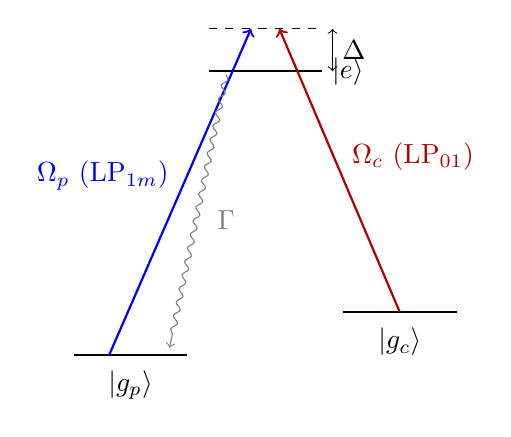
\begin{tikzpicture}[scale=0.9]
\draw[thick] (-0.2,0)--(1.4,0) node[below=2pt,midway]{$\gp$};
\draw[thick] (3.6,0.6)--(5.2,0.6) node[below=2pt,midway]{$\gc$};
\draw[thick] (1.7,4)--(3.3,4) node[right]{$\ket e$};
\draw[dashed] (1.7,4.6)--(3.3,4.6);
\draw[->,thick,blue] (0.3,0)--(2.3,4.6) node[pos=0.55,left=3pt]{$\Om_p$ (LP$_{1m}$)};
\draw[->,thick,red!70!black] (4.4,0.6)--(2.7,4.6) node[pos=0.55,right=3pt]{$\Om_c$ (LP$_{01}$)};
\draw[<->] (3.45,4)--(3.45,4.6) node[midway,right]{$\Delta$};
\draw[->,gray,decorate,decoration={snake,amplitude=1pt,segment length=5pt,post length=3pt}] (1.95,3.95)--(1.15,0.1);
\node[gray] at (1.95,1.9) {$\Gamma$};
\end{tikzpicture}\hspace{1.2cm}
\begin{tikzpicture}
\begin{axis}[width=0.5\textwidth,height=0.36\textwidth,xlabel={two-photon detuning $\delta/2\pi$ (kHz)},
  ylabel={$R(\delta)/R(\delta_+)$},xmin=-12,xmax=12,ymin=0,ymax=1.05]
\addplot[black,thick] table[x=d,y=R]{../../simulation/results/report/fano.dat};
\draw[blue,dashed] (axis cs:5,0)--(axis cs:5,1.05);
\draw[red,dashed] (axis cs:-5,0)--(axis cs:-5,1.05);
\node[blue,font=\scriptsize,anchor=west] at (axis cs:5.3,0.6) {$A_-$};
\node[red,font=\scriptsize,anchor=east] at (axis cs:-5.3,0.6) {$A_+$};
\end{axis}
\end{tikzpicture}
\caption{Left: $\Lambda$ scheme with the probe in an LP$_{1m}$ mode and the coupling beam in LP$_{01}$. Right: Fano absorption profile, Eq.~\eqref{eq:fano}, for $\nu=2\pi\times\SI{5}{kHz}$, $\Delta=3\Gamma$ and $\Om_c^2/4\Delta=\nu$. The red sideband ($A_-$, cooling) sits on the narrow peak, the carrier on the zero, and the blue sideband ($A_+$) is suppressed by $(\Gamma/4\Delta)^2\approx7\times10^{-3}$.}
\label{fig:fano}
\end{figure}

\subsection{Rate equation}
In the secular, weak-probe limit, the absorption rates on the red and blue sidebands are $A_\mp=\etaeff^2R(\pm\nu)$. Set the EIT condition $\Om_c^2/4\Delta=\nu$. Then $A_-$ sits on the narrow peak and the carrier ($\delta=0$) on the transparency zero. Every absorbed probe photon is followed by a spontaneous emission that deposits on average $\alpha\eta_{\rm sp}^2$ quanta in the radial mode considered. Here $\eta_{\rm sp}=k x_0$ and $\alpha\approx2/5$ for a $\pi$ dipole and an axis perpendicular to it. Because $E_{\rm rec}/\hbar\nu=\eta_{\rm sp}^2$, this holds exactly for the mean energy even though radially $\eta_{\rm sp}\sim0.3$--$0.7$ is not small. For the node geometry, where all probe scattering is sideband scattering,
\begin{equation}
  \frac{d\langle n\rangle}{dt}=-A_-\langle n\rangle(1-\alpha\eta_{\rm sp}^2)+A_+(\langle n\rangle+1)(1+\alpha\eta_{\rm sp}^2),
  \label{eq:rate}
\end{equation}
\begin{equation}
  W=A_-(1-\alpha\eta_{\rm sp}^2)-A_+(1+\alpha\eta_{\rm sp}^2),\qquad
  n_{\rm ss}=\frac{A_+(1+\alpha\eta_{\rm sp}^2)}{W}\simeq\Big(\frac{\Gamma}{4\Delta}\Big)^2\frac{1+\alpha\eta_{\rm sp}^2}{1-\alpha\eta_{\rm sp}^2}.
  \label{eq:nss}
\end{equation}
If the probe also drives the carrier (any geometry without a node), Eq.~\eqref{eq:rate} acquires the familiar additional heating term $+\alpha\eta_{\rm sp}^2R_{\rm car}(\delta_{\rm err})$, where $R_{\rm car}$ is the carrier scattering rate at the residual two-photon detuning $\delta_{\rm err}$~\cite{leibfried2003,eschner2003}. EIT cancels these only at exact two-photon resonance. The node geometry removes them for any $\delta_{\rm err}$, which makes it robust against inhomogeneous differential light shifts of the lattice.

Equation~\eqref{eq:nss} shows the two points specific to the radial direction. First, recoil heating is large: $\alpha\eta_{\rm sp}^2\approx0.2$ for $\nu_r=\SI{7}{kHz}$. It is still below unity, so every cooling cycle removes net energy. Second, the Fano limit $(\Gamma/4\Delta)^2$ is the same as in ion experiments~\cite{morigi2000,roos2000,lechner2016}. EIT cooling of neutral atoms in lattices and dipole traps has been demonstrated~\cite{haller2015,kampschulte2014}, as has a double-bright variant that addresses two widely separated frequencies~\cite{scharnhorst2018}. Double-EIT can additionally suppress blue-sideband heating~\cite{evers2004}.

\subsection{Rate ceilings: $\eta^2$-limited versus resolution-limited}
\label{sec:ceilings}
The cooling rate is $A_-\simeq\etaeff^2\bar\Om_p^2/\Gamma=\Om_\perp^2/\Gamma$. How large $\Om_\perp$ can be depends on whether the probe also drives the carrier:

\textbf{(i) Carrier present} (conventional EIT, or a probe that is a superposition of LP$_{01}$ and LP$_{1m}$, e.g.\ for simultaneous axial and radial action). The probe Rabi frequency at the atom must stay perturbative, $\bar\Om_p\lesssim\Om_c/3$, to keep the Fano structure intact~\cite{morigi2003}. Using $\Om_c^2=4\Delta\nu$,
\begin{equation}
  W_{\rm std}\simeq\frac{4\Delta}{9\Gamma}\,\etaeff^2\,\nu
  =\frac{4\Delta}{9\Gamma}\,G_{1m}^2\,\frac{\hbar}{2m_{\rm Rb}a^2}.
  \label{eq:Wstd}
\end{equation}
Because $\etaeff^2\nu=G_{1m}^2\hbar/2m_{\rm Rb}a^2$, this ceiling does not depend on the trap frequency. It is set entirely by the ``transverse recoil frequency'' of the core, which is only $\hbar/2m_{\rm Rb}a^2=\SI{1.6}{s^{-1}}$ for $a=\SI{15}{\micrometre}$.

\textbf{(ii) Node geometry.} The atom never sees the carrier field, so $\bar\Om_p$ can be raised until the sideband coupling itself saturates the narrow resonance. Treating the narrow dressed state as a two-level transition of width $\Gamma_n$ gives
\begin{equation}
  A_-=\frac{\Om_\perp^2/\Gamma}{1+s},\quad s=\frac{2\Om_\perp^2}{\Gamma\Gamma_n}
  \quad\Rightarrow\quad W_{\rm node}\lesssim\frac{\Gamma_n}{2},\ \text{ typically }\frac{\Gamma_n}{4}\ (s=1).
  \label{eq:Wnode}
\end{equation}
Resolution requires $\Gamma_n\lesssim\nu$. With $\Gamma_n=\Gamma\nu/\Delta$ and $\Delta=3\Gamma$, we get $W_{\rm node}\approx\nu_r/12$. This bound does not depend on $\etaeff$: the small geometric factor appears only as the required probe power, $P\propto(a/G_{1m}x_0)^2$.

\begin{table}[t]
\centering
\caption{Estimates for an ideal $\Lambda$ system on the $^{87}$Rb D1 line, with a \SI{1064}{nm} lattice, $\nu_z=\SI{300}{kHz}$, $\Delta=3\Gamma$, $\Om_c^2/4\Delta=\nu_r$ and an LP$_{11}$ probe ($G=3.49$). $P_{\rm probe}$ is the LP$_{11}$ power for $s=1$, using $I_{\rm sat}\approx\SI{4.5}{mW/cm^2}$~\cite{steck87}. Multilevel structure, imperfect pumping and technical heating will lower the rates. Read them as upper limits.}
\label{tab:numbers}
\begin{tabular}{lcc}
\toprule
& kagome/ARF, $2a=\SI{30}{\micrometre}$ & PBG, $2a=\SI{7}{\micrometre}$\\
\midrule
$\nu_r/2\pi$ & \SI{7.1}{kHz} & \SI{31}{kHz}\\
$x_0$ & \SI{90}{nm} & \SI{44}{nm}\\
$\etaeff$ (LP$_{11}$) & 0.021 & 0.044\\
$\eta_{\rm sp}$ / recoil per photon $\alpha\eta_{\rm sp}^2$ & 0.71 / 0.20 & 0.34 / 0.05\\
$\Om_c/2\pi$, $\Gamma_n/2\pi$ & \SI{0.70}{MHz}, \SI{2.4}{kHz} & \SI{1.45}{MHz}, \SI{10}{kHz}\\
$W_{\rm std}$, Eq.~\eqref{eq:Wstd} & $\approx\SI{26}{s^{-1}}$ & $\approx\SI{490}{s^{-1}}$\\
$W_{\rm node}$, Eq.~\eqref{eq:Wnode} & $\approx\SI{3.7\times10^{3}}{s^{-1}}$ & $\approx\SI{1.6\times10^{4}}{s^{-1}}$\\
$P_{\rm probe}$ (node, $s=1$) & $\approx\SI{8}{nW}$ & $\approx\SI{0.4}{nW}$\\
$n_{\rm ss}$ (Fano + recoil) & $\approx0.010$ & $\approx0.008$\\
\bottomrule
\end{tabular}
\end{table}

Table~\ref{tab:numbers} shows the difference between the two regimes. With a carrier present, radial cooling in a large-core fibre runs at a few tens of s$^{-1}$. That competes poorly with lattice photon scattering and technical heating~\cite{savard1997,grimm2000}. In the node geometry the ideal ceiling is two orders of magnitude higher, and the probe power needed is negligible. The $n_{\rm ss}$ values are ideal-$\Lambda$ limits. In practice the floor will be set by imperfect pumping, residual carrier from mode impurity or atom displacement, and technical heating (Sec.~\ref{sec:practical}).

%=====================================================================
\section{Spontaneous emission inside the hollow core}
\label{sec:emission}
%=====================================================================
The cooling theory above treats spontaneous emission as in free space. It assumes a total decay rate $\Gamma$, a recoil drawn from the dipole radiation pattern, and photons that never return. The master-equation simulations of the paper make the same assumptions. Inside a fibre the atom radiates into a structured electromagnetic environment that guides only a few modes, so the assumptions need checking. We ask three questions. Does the fibre change the decay rate (Purcell effect)? Does it change the recoil distribution? What happens to the photons that stay in the fibre? In short: a single atom on the axis of a hollow core with $ka\gg1$ radiates almost as in free space, with corrections of a few per cent. The fibre matters mainly collectively, through the large optical depth of the atomic column in the guided modes. Table~\ref{tab:emission} collects the numbers.

\subsection{Guided fraction of the emission}
A photon stays in the fibre only if it is emitted into one of the few low-loss core modes, i.e.\ into a narrow cone around the axis. All other directions hit the core wall at angles where it reflects weakly, and that light leaves through the cladding. A linear dipole matched to the polarisation of a mode with transverse profile $\psi$, normalised to $\int|\psi|^2dA=1$, emits into one propagation direction of that mode with the fraction~\cite{lekien2005}
\begin{equation}
  \frac{\Gamma_{\rm mode}}{\Gamma}=\frac{3\lambda^2}{8\pi}\,|\psi(\mathbf r_0)|^2
  \quad\Rightarrow\quad
  \beta_{01}=\frac{3\lambda^2}{8\pi^2a^2J_1^2(u_{01})}\approx0.14\,\frac{\lambda^2}{a^2}
  \label{eq:beta01}
\end{equation}
for LP$_{01}$ and an atom on the axis (group velocity $\simeq c$). This gives $\beta_{01}=4\times10^{-4}$ for $a=\SI{15}{\micrometre}$ and $7\times10^{-3}$ for $a=\SI{3.5}{\micrometre}$. On the axis only the LP$_{0m}$ modes receive light, because all LP$_{lm}$ with $l\ge1$ have a node there. Summed over the LP$_{0m}$ modes that remain low-loss, the guided fraction is the emission of a transverse dipole into a cone of half-angle $\theta_g\approx u_{0m,\max}/ka$ in both directions:
\begin{equation}
  f_g\simeq\tfrac34\,\theta_g^2 .
  \label{eq:fg}
\end{equation}
This gives $f_g\approx(2$--$4)\times10^{-3}$ for case A (LP$_{01}$--LP$_{03}$) and $(1.5$--$3)\times10^{-2}$ for case B (LP$_{01}$--LP$_{02}$). The polarisation matters as well. In the weak-guidance limit the LP$_{0m}$ fields are transverse and have no longitudinal component on the axis. A dipole along the fibre axis, which is the orientation assumed for the recoil in the simulations, therefore emits into guided modes only at a further reduced level $\sim(u/ka)^2$. In every case, more than 97\% of the light leaves the core as it would in free space. This is the essential difference from nanofibres, where the atom sits in the evanescent field of a sub-wavelength guide and $\beta$ reaches a few tens of per cent~\cite{lekien2005,chang2018}. A hollow core with $a\gg\lambda$ is a weak-coupling waveguide: its strength lies in the collective coupling of many atoms (Sec.~\ref{sec:collective}), not in the single-atom $\beta$.

\subsection{Total decay rate}
The decay rate is set by the local density of optical states at the atom, which a nearby boundary can raise or lower~\cite{kleppner1981}. Here the boundary is far away ($ka=118$ and 28 for the two cases) and reflects weakly. At normal incidence the amplitude reflection coefficient is $|r_\perp|=0.18$ for bulk silica and up to 0.35 for a thin silica membrane. The cylindrical shape gives one specific feature: light emitted perpendicular to the axis is reflected back onto the axis from the whole circumference, so the reflected wave refocuses on the atom. We expand the dipole field in cylindrical waves $H_0^{(1)}(k_\perp\rho)e^{i\beta z}$ and reflect each with its Fresnel coefficient. Evaluating the returning field at the stationary phase $\beta=0$ gives, for a dipole along the axis on the axis,
\begin{equation}
  \frac{\Delta\Gamma}{\Gamma}\simeq\frac32\,|r_\perp|\sqrt{\frac{\pi}{ka}}\,
  \sin\!\big(2ka+\varphi_r-\tfrac{\pi}{4}\big).
  \label{eq:purcell}
\end{equation}
A transverse dipole gives a result of the same order. The full integral over $\beta$, including multiple reflections, agrees with Eq.~\eqref{eq:purcell}. With the angle-dependent Fresnel coefficients and $a$ varied over $\lambda/2$, it gives $\Delta\Gamma/\Gamma$ between $-4\%$ and $+5\%$ for a bulk-silica wall with $a=\SI{15}{\micrometre}$, and up to $\pm9\%$ for membranes of thickness 0.2--\SI{0.7}{\micrometre}. For $a=\SI{3.5}{\micrometre}$ the range is $\pm10\%$ for bulk silica and up to $-14\%$ to $+22\%$ for membranes. In practice the correction is smaller, for three reasons:
\begin{itemize}
\item It oscillates with period $\lambda/2$ in $a$ and so depends on sub-wavelength details of the core shape.
\item It varies across the atom on the scale $1/2k$. For an atom in the radial ground state it is reduced by $\approx e^{-2\eta_{\rm sp}^2}$ (0.36 for A, 0.79 for B), and at \SI{10}{\microkelvin} it averages out.
\item A nested antiresonant fibre has no continuous cylindrical wall. Its cladding tubes are convex towards the core and defocus the reflected light.
\end{itemize}
The estimate therefore applies best to bandgap and capillary cores, i.e.\ to case B.

For cooling, a modified $\Gamma$ is a constant renormalisation. The dark state does not involve $\Gamma$, and $\Delta$, $\Gamma_n$ and $s$ are set experimentally from the measured linewidth anyway. The two legs of the $\Lambda$ system share the excited state. Because they have different polarisations, however, the branching ratio $b_p$ can shift at the per-cent level. That enters only through the photon number per cycle, $\kappa=1/b_p$. The fibre also introduces no memory effects. The round trip to the wall, $2a/c\lesssim\SI{0.1}{ps}$, and even that to a fibre facet \SI{10}{cm} away, \SI{0.7}{ns}, are far shorter than $1/\Gamma=\SI{27}{ns}$. Facet reflections act only on the small guided fraction. The Markovian free-space master equation is therefore appropriate.

\subsection{Recoil}
\label{sec:emission-recoil}
The radial recoil per photon, $\alpha\eta_{\rm sp}^2$ in Eq.~\eqref{eq:rate}, comes from the dipole pattern ($\alpha\approx2/5$ for $x$ perpendicular to the dipole). A guided photon carries transverse momentum $\sim\hbar u_{0m}/a\ll\hbar k$, so the guided fraction lowers the radial recoil by at most $f_g$, i.e.\ 0.4\% for A and 3\% for B. The wall reflections make the direct and reflected emission interfere. This is the atom--mirror-image interference observed with single ions~\cite{eschner2001}. It redistributes the photons around $\theta=\pi/2$ but changes $\langle k_x^2\rangle$ only at the level of $\Delta\Gamma/\Gamma$. The recoil model of the simulations thus holds to within a few per cent. The fibre gives no reduction of the recoil heating, unlike a high-$\beta$ waveguide or a cavity, where most photons could be emitted along the axis.

The node geometry has one curious consequence. Because $\psi_{11}$ vanishes on the axis and grows linearly with $x$, an atom emits into LP$_{11}$ only when its radial vibrational number changes by one. This is the time reverse of the probe coupling. Guided LP$_{11}$ fluorescence is thus pure sideband light, with the fraction $2\beta_{01}\etaeff^2(2\langle n\rangle+1)$ per emitted photon. That is $4\times10^{-7}$ (A) and $3\times10^{-5}$ (B) in the ground state: negligible as a heating channel and too weak for thermometry with a single atom.

\subsection{Collective effects: reabsorption and probe depletion}
\label{sec:collective}
The single-atom $\beta_{01}$ is small, but the guided mode is shared by the whole column. On a two-level transition with $\sigma_0=3\lambda^2/2\pi$, the resonant optical depth of $N$ atoms in LP$_{01}$ is $\mathrm{OD}=4N\beta_{01}$. For $N=10^4$ this is $\approx16$ (A) and $\approx290$ (B), before D1 Clebsch--Gordan factors. Optical depths of this size have been measured in hollow-core fibres~\cite{blatt2014}.

\paragraph{Reabsorption of cooling photons.} There is a point specific to EIT cooling. In a cooling cycle the atom absorbs a red-sideband probe photon and returns to $\gp$ on the motional carrier. The emitted photon then has frequency $\omega_p+\nu_r$, which coincides with the narrow resonance $\delta_+=\nu_r$ of every other atom in the dark state. There the peak cross-section is the full $\sigma_0$ [Eq.~\eqref{eq:narrow}]. Photons emitted towards $\gc$ meet an almost empty coupling transition, and photons emitted on a motional sideband fall on the transparency zero ($\delta=0$) or at $\delta=2\nu_r$, so these pass. A fraction $\approx b_p(1-\alpha\eta_{\rm sp}^2)$ of the scattered light is therefore resonant with the ensemble. Two channels bring it back to the atoms:
\begin{itemize}
\item the guided fraction $f_g$, which is almost surely reabsorbed when OD\,$\gg1$;
\item the light reflected by the wall, which refocuses onto the axis. Weighted by the dipole pattern, the reflected fraction is $\bar R\approx2$--9\% (bulk silica to membranes). A converging cylindrical wave meets a line of absorbers with linear density $\rho_l$ and is absorbed with probability $\approx\min(1,3\lambda\rho_l)$, which is close to 1 for $\sim1$ atom per \si{\micro m}.
\end{itemize}
Hence the reabsorption probability per emitted photon is
\begin{equation}
  p_{\rm re}\lesssim b_p(1-\alpha\eta_{\rm sp}^2)\,(f_g+\bar R)\approx4\%\ \text{(A)},\ 6\%\ \text{(B)}.
\end{equation}
A reabsorbed photon is absorbed on the narrow resonance, whose width $\Gamma_n=\nu_r/3$ resolves the motional sidebands. For the absorbing atom, the sidebands lie at $\delta=2\nu_r$ (off resonance) and $\delta=0$ (dark), so the absorption happens on the motional carrier. This is the festina-lente regime, in which reabsorption heating is suppressed~\cite{castin1998}. Only the recoil of the re-emitted photon heats, so the rate is reduced by
\begin{equation}
  \frac{\Delta W}{W}\approx-\frac{\kappa\,p_{\rm re}\,\alpha\eta_{\rm sp}^2}{1-\kappa\alpha\eta_{\rm sp}^2}\approx-3\%\ \text{(A)},\ -0.6\%\ \text{(B)}
\end{equation}
with $\kappa=2$, and $n_{\rm ss}$ grows by the same relative amount. For atom numbers of order $10^4$, reabsorption is thus a small correction. It would grow mainly through $\bar R$, i.e.\ with a strongly reflecting core surround. Unlike free space, it is dominated by the refocusing wall rather than by the density of the cloud.

\paragraph{Probe depletion.} The same collective coupling acts on the LP$_{11}$ probe, which loses one photon per sideband absorption. An atom absorbs at most $\sim\Gamma_n/2$ probe photons per second (saturated narrow line), so the probe must carry at least $P_{\min}\approx N\hbar\omega\,\Gamma_n/2$. For $N=10^4$ this is \SI{0.02}{nW} (A) and \SI{0.08}{nW} (B), compared with \SI{8}{nW} and \SI{0.4}{nW} needed for $s=1$ (Table~\ref{tab:numbers}). In case A depletion is negligible. In case B up to $\sim20\%$ of the probe is absorbed while the hot thermal tail is cooled, so the saturation parameter falls along the column. Raising the probe power or launching it from both ends compensates for this. Near the ground state the absorption vanishes, because the red-sideband rate is $\propto\langle n\rangle$.

\begin{table}[t]
\centering
\caption{Emission inside the hollow core compared with free space, for an atom on the axis at \SI{795}{nm}. The free-space values are $\beta=0$, $\Delta\Gamma=0$ and no reabsorption. Ranges for $\Delta\Gamma/\Gamma$ cover bulk-silica and membrane walls of a continuous cylindrical core surround, with $a$ varied over $\lambda/2$; nested-tube claddings give less. Reabsorption assumes $N=10^4$, $\sim1$ atom/\si{\micro m}, $b_p=1/2$ and $\kappa=2$.}
\label{tab:emission}
\small
\begin{tabular}{lcc}
\toprule
& case A, $a=\SI{15}{\micrometre}$ & case B, $a=\SI{3.5}{\micrometre}$\\
\midrule
$ka$ & 118 & 28\\
$\beta_{01}$ per direction, Eq.~\eqref{eq:beta01} & $4.0\times10^{-4}$ & $7.3\times10^{-3}$\\
guided fraction $f_g$ (all low-loss LP$_{0m}$) & $(2$--$4)\times10^{-3}$ & $(1.5$--$3)\times10^{-2}$\\
$\Delta\Gamma/\Gamma$ (wall refocusing) & $\pm(4$--$9)\%$ & $\pm(10$--$20)\%$\\
\quad averaged over radial ground state & $\times0.36$ & $\times0.79$\\
change of radial recoil per photon & $\lesssim0.4\%$ & $\lesssim3\%$\\
OD in LP$_{01}$ (two-level, $N=10^4$) & 16 & 290\\
reabsorption probability $p_{\rm re}$ & $\lesssim4\%$ & $\lesssim6\%$\\
resulting change of $W$ and $n_{\rm ss}$ & $\lesssim3\%$ & $\lesssim1\%$\\
minimum probe power for $N=10^4$ & \SI{0.02}{nW} & \SI{0.08}{nW}\\
\bottomrule
\end{tabular}
\end{table}

\subsection{What changes with respect to free space}
\begin{enumerate}
\item \textbf{Decay rate:} essentially unchanged. The wall changes $\Gamma$ by a few per cent (up to $\sim$10--20\% for a perfectly circular small core). The change acts as a constant that is calibrated in situ.
\item \textbf{Mode selectivity:} only a cone of half-angle $\sim u/ka$ is guided, i.e.\ $10^{-3}$--$10^{-2}$ of the light. An atom on the node does not emit into LP$_{l\ge1}$ modes at all, except through motional sidebands. More than 97\% of the photons leave sideways as in free space.
\item \textbf{Recoil:} free-space dipole pattern to within a few per cent. The free-space recoil model of the master equation is adequate, and the fibre offers no reduction of recoil heating.
\item \textbf{Collective coupling:} this is what really changes. The column has an optical depth of tens to hundreds in the guided modes, and the wall refocuses side-scattered light onto the axis. Cooling photons are resonant with the narrow EIT line of the other atoms. Reabsorption costs only a few per cent of the rate, because $\Gamma_n<\nu_r$ suppresses heating on reabsorption. In small cores with many atoms, the probe photon budget becomes relevant.
\end{enumerate}

%=====================================================================
\section{Trends and scaling laws}
\label{sec:trends}
%=====================================================================
Combining Eqs.~\eqref{eq:freqs}, \eqref{eq:etaeff}, \eqref{eq:Wstd} and \eqref{eq:Wnode}:
\begin{align}
  \nu_r&\propto\frac{\sqrt{U_0}}{a}, &
  \etaeff&\propto\frac{G_{1m}}{a\sqrt{\nu_r}}\propto\frac{G_{1m}}{\sqrt a\,U_0^{1/4}}, &
  \alpha\eta_{\rm sp}^2&\propto\frac1{\nu_r}\propto\frac{a}{\sqrt{U_0}},\nonumber\\
  W_{\rm std}&\propto\frac{\Delta}{\Gamma}\frac{G_{1m}^2}{a^2}, &
  W_{\rm node}&\simeq\frac{\Gamma}{4\Delta}\nu_r\propto\frac{\sqrt{U_0}}{a}, &
  P_{\rm probe}&\propto\frac{a^4\nu_r^2}{G_{1m}^2}.
  \label{eq:scaling}
\end{align}
Five trends follow (Fig.~\ref{fig:trend}):
\begin{itemize}
\item \textbf{Core size} is the most important design parameter. $W_{\rm std}$ scales as $a^{-2}$ and $W_{\rm node}$ as $a^{-1}$. A smaller core also lowers the radial recoil heating per photon. Its limit is fibre loss, which grows as $a^{-3}$ and degrades probe-mode purity (Sec.~\ref{sec:coresize}).
\item \textbf{Lattice depth} raises $\nu_r$, and with it $W_{\rm node}$ and the recoil budget. It leaves $W_{\rm std}$ unchanged, but it also increases lattice photon scattering and differential light shifts.
\item \textbf{Single-photon detuning} $\Delta$ trades rate against the Fano floor: $W_{\rm node}\propto1/\Delta$ and $n_{\rm ss}\propto1/\Delta^2$. In the carrier regime a larger $\Delta$ helps, since $W_{\rm std}\propto\Delta$, until $W_{\rm std}$ reaches the $\Gamma_n$ ceiling.
\item \textbf{Mode order} enters only $W_{\rm std}$ (as $G_{1m}^2\propto u_{1m}^3$) and the required power. It does not enter the node-geometry ceiling.
\item Both axial and radial cooling need the Fano peak at the relevant frequency. Since $\nu_z/\nu_r\sim40$, a single coupling setting cannot serve both. Use time-multiplexed stages or a double-bright scheme~\cite{scharnhorst2018}.
\end{itemize}

\begin{figure}[t]
\centering
\begin{tikzpicture}
\begin{axis}[width=0.7\textwidth,height=0.45\textwidth,xlabel={core radius $a$ (\si{\micrometre})},
  ylabel={cooling-rate ceiling $W$ (s$^{-1}$)},ymode=log,xmin=3,xmax=32,ymin=1,ymax=1e5,
  legend style={font=\scriptsize,at={(0.98,0.98)},anchor=north east},legend cell align=left]
\addplot[black,very thick] table[x=a,y=Wnode]{../../simulation/results/report/trend_a.dat};
\addplot[blue,thick] table[x=a,y=Wstd1]{../../simulation/results/report/trend_a.dat};
\addplot[red!70!black,thick] table[x=a,y=Wstd3]{../../simulation/results/report/trend_a.dat};
\addplot[orange!80!black,thick] table[x=a,y=Wstd5]{../../simulation/results/report/trend_a.dat};
\legend{node geometry ($\Gamma_n/4$; any $m$),carrier regime LP$_{11}$,carrier regime LP$_{13}$,carrier regime LP$_{15}$}
\end{axis}
\end{tikzpicture}
\caption{Ideal-$\Lambda$ radial cooling-rate ceilings versus core radius, for $\nu_z=\SI{300}{kHz}$ (\SI{1064}{nm} lattice) and $\Delta=3\Gamma$. In the carrier regime the rate scales as $G_{1m}^2/a^2$ and is capped by the resolution limit $\Gamma_n/4$ (black curve). The node geometry reaches that cap for any $m$ given enough probe power, which is only nW.}
\label{fig:trend}
\end{figure}

%=====================================================================
\section{Very high-order modes}
\label{sec:hom}
%=====================================================================
With $G_{1m}\simeq0.46u_{1m}^{3/2}$ and $u_{1m}\simeq(m+\tfrac14)\pi$, the effective radial Lamb--Dicke parameter grows as $m^{3/2}$:
\begin{equation}
  \etaeff\simeq0.46\,u_{1m}^{3/2}\frac{x_0}{a},\qquad
  W_{\rm std}\propto u_{1m}^3,\qquad P_{\rm probe}\propto u_{1m}^{-3}.
\end{equation}
Going from LP$_{11}$ to LP$_{15}$ raises $\etaeff$ by a factor 8.8. For $a=\SI{15}{\micrometre}$ that takes $W_{\rm std}$ from $\sim\SI{26}{s^{-1}}$ to $\sim\SI{2\times10^{3}}{s^{-1}}$, close to the resolution ceiling.

\subsection{Benefits}
\begin{enumerate}
\item \textbf{Carrier regime.} The rate grows as $u_{1m}^3$, which makes simultaneous axial and radial probing with one superposed probe viable.
\item \textbf{Node regime.} The rate does not increase, but the probe power falls as $u_{1m}^{-3}$. More importantly, the tolerance to mode impurity improves. If the probe contains a fraction $\epsilon$ (in amplitude) of LP$_{01}$, the carrier-to-sideband ratio is $\epsilon a/(G_{1m}x_0)=\epsilon/\etaeff$. The carrier is dark, but it caps the usable probe power, and the node ceiling survives only for $\epsilon\lesssim2.8\,\etaeff$ (Sec.~\ref{sec:coresize}). For LP$_{11}$ at $a=\SI{15}{\micrometre}$ this means $\epsilon\lesssim0.06$ (power impurity $\lesssim0.4\%$); for LP$_{15}$ it relaxes to $\epsilon\lesssim0.5$.
\item The node always sits on the fibre axis, independent of $m$, so the alignment advantage is kept.
\end{enumerate}

\subsection{Costs}
\begin{enumerate}
\item \textbf{Capture range.} The linear approximation needs $(u_{1m}x/a)^2/8\ll1$. Atoms with $\langle n\rangle\gtrsim n_{\rm lin}=0.4(a/u_{1m}x_0)^2$ (Table~\ref{tab:G}) reach the curvature of the first lobe or the first ring node, where the coupling weakens and changes sign. For $a=\SI{15}{\micrometre}$, LP$_{15}$ is efficient only below $\langle n\rangle\approx30$, whereas a \SI{10}{\microkelvin} sample has $\langle n_r\rangle\approx30$--$40$. This suggests a \emph{cascade}: start with LP$_{11}$ (large capture range) and switch to higher $m$ (stronger, more robust coupling) as the atoms cool.
\item \textbf{Loss and filtering.} HOM loss grows at least as $u_{1m}^2$~\cite{marcatili1964}. Fibres designed to be effectively single-mode strip HOMs resonantly~\cite{uebel2016,poletti2014}. The propagation angle $\theta_m\approx u_{1m}/ka$ (0.14\,rad for LP$_{15}$ at $a=\SI{15}{\micrometre}$) approaches the range where cladding resonances dominate. Short fibre sections, or injecting the probe from the end close to the atoms, mitigate this. Section~\ref{sec:coresize} quantifies the resulting trade-off with core size.
\item \textbf{Excitation and purity.} Clean LP$_{1m}$ excitation needs a phase plate or SLM with radial and azimuthal phase structure. Intermodal crosstalk at splices, bends and the fibre entrance feeds LP$_{01}$ (carrier) and other $l$ components.
\item \textbf{Vector-mode structure.} TE/TM/HE splitting and birefringence rotate the lobe pattern and alter the local polarisation along the fibre~\cite{snyder1983,ramachandran2013}. A rotating lobe pattern does mix $x$ and $y$ cooling across lattice sites, which can help. A polarisation that varies across the core breaks the clean $\Lambda$ system and populates bright Zeeman states.
\item \textbf{Beating.} A pure LP$_{1m}$ probe does not interfere with itself. Any LP$_{01}$ admixture, however, beats with period $L_B\propto a^2/u_{1m}^2$ ($\approx\SI{80}{\micrometre}$ for LP$_{15}$). This moves the effective node off axis at some sites and makes the carrier contamination site-dependent.
\end{enumerate}

Modes with $l\ge2$ vanish as $r^l$ on axis and give no first-order coupling, so the useful family is $l=1$. LP$_{11}^{e}$ and LP$_{11}^{o}$ cool $x$ and $y$ respectively; alternate between them or rely on trap anisotropy to mix the two axes. A single OAM $\ell=\pm1$ mode, $\propto x\pm iy$, couples to only one circular combination at the red-sideband frequency. It is not by itself a substitute for two orthogonal lobes.

%=====================================================================
\section{Core size, fibre length and the number of usable modes}
\label{sec:coresize}
%=====================================================================
Sections~\ref{sec:trends} and~\ref{sec:hom} point in two directions. A smaller core raises $\nu_r$ and every rate ceiling. A higher mode order raises $\etaeff$. But the number of modes a fibre transmits over a given length grows with the core size. This section asks whether that creates an optimum core radius, and what sets it.

\subsection{Loss budget and mode count}
We keep the Marcatili scaling of Eq.~\eqref{eq:beta} for the power attenuation and write it relative to the fundamental mode:
\begin{equation}
  \alpha_{lm}(a)=\alpha_{01}(a)\left(\frac{u_{lm}}{u_{01}}\right)^2,\qquad
  \alpha_{01}(a)=A_{15}\left(\frac{\SI{15}{\micrometre}}{a}\right)^3 .
  \label{eq:lossmodel}
\end{equation}
$A_{15}$ is the LP$_{01}$ loss of the fibre type at $a=\SI{15}{\micrometre}$ and $\lambda=\SI{795}{nm}$. For a bare silica capillary, the exact Marcatili EH-mode loss~\cite{marcatili1964} gives $A_{15}\approx\SI{350}{dB/m}$. Inhibited coupling lowers this by orders of magnitude. A hypocycloid kagome fibre with \SI{40}{\micrometre} core diameter reaches \SI{70}{dB/km} near \SI{800}{nm}~\cite{bradley2013}, which scales to $A_{15}\approx\SI{0.17}{dB/m}$. In inhibited-coupling fibres the dependence on $a$ and $\lambda$ is design dependent and often steeper than $a^{-3}$~\cite{fokoua2023,zeisberger2017}. We therefore treat $A_{15}$ as the free parameter that encodes fibre quality.

The $u_{lm}^2$ factor is a fair guide for kagome fibres. Measured LP$_{11}$/LP$_{01}$ loss ratios are 2.6--3.6 and the LP$_{21}$ ratio is 5.7~\cite{bradley2016}; Eq.~\eqref{eq:lossmodel} gives 2.5 and 4.6. One exception is LP$_{02}$ in a 19-cell fibre, measured at 2.6 against a predicted 5.3.

The number of modes that survive a length $L$ with $\alpha_{lm}L<1$ follows from the Weyl count of a disk: $u_{lm}<u_{\max}=u_{01}/\sqrt{\alpha_{01}L}$. Including both polarisations,
\begin{equation}
  N(L)\simeq\frac{u_{\max}^2}{2}=\frac{u_{01}^2}{2\,\alpha_{01}(a)\,L}\ \propto\ \frac{a^3}{\lambda^2L}.
  \label{eq:modecount}
\end{equation}
This confirms the premise: a twice larger core transmits about eight times as many modes. For the kagome-like loss, $N\approx250$ for $a=\SI{15}{\micrometre}$ and $L=\SI{30}{cm}$. For a bare capillary the figure is $N<1$, and $N$ reaches about 6 only at $a=\SI{30}{\micrometre}$, $L=\SI{5}{cm}$.

In real microstructured fibres the cladding, not the loss, usually caps the mode count. A core mode with transverse wavenumber $u_{lm}/a$ is stripped when it phase-matches a cladding-hole or tube mode, $u_{lm}/a\approx u_{01}/r_c$~\cite{uebel2016}. Seven- and 19-cell kagome fibres guide only 4 and 7 LP mode groups~\cite{bradley2016}, i.e.\ at most LP$_{11}$ and LP$_{12}$ in the $l=1$ family. Keeping LP$_{1m}$ guided needs $r_c/a\lesssim u_{01}/u_{1m}$: 0.34 for LP$_{12}$ and 0.15 for LP$_{15}$. For a single ring of $N_t$ touching tubes around an inscribed core of radius $a$, $r_t/a=\sin(\pi/N_t)/[1-\sin(\pi/N_t)]$. LP$_{12}$ then needs $N_t\gtrsim13$ tubes and LP$_{15}$ needs $N_t\gtrsim25$. These are HOM-\emph{preserving} designs, the opposite of the usual single-mode optimisation.

\subsection{Mode purity along the fibre and the optimum mode index}
Loss matters for the node scheme because it degrades mode purity, not because of power: only nW are needed. Suppose the probe is launched as LP$_{1m}$ with a residual LP$_{01}$ amplitude $\epsilon_0$; with a phase plate or SLM, $\epsilon_0\approx0.03$--0.1, i.e.\ $-30$ to $-20$\,dB. LP$_{01}$ has the lower loss, so its relative amplitude grows along the fibre:
\begin{equation}
  \epsilon(z)=\epsilon_0\exp\!\left[\tfrac12(\alpha_{1m}-\alpha_{01})z\right].
  \label{eq:epsz}
\end{equation}
LP$_{0m'}$ modes with $u_{0m'}<u_{1m}$ act in the same way, and so does crosstalk from bends and splices, so Eq.~\eqref{eq:epsz} is optimistic.

The admixed carrier sits at the dark resonance, $R(0)=0$, so it does not heat directly. It does, however, cap the probe field at $\epsilon\bar\Om_p\lesssim\Om_c/3$, the same condition as in regime (i) of Sec.~\ref{sec:ceilings}. That limits the sideband saturation parameter to $s\le s_{\rm car}=8(\Delta/3\Gamma)^2(\etaeff/\epsilon)^2$. Equations~\eqref{eq:Wstd} and~\eqref{eq:Wnode} then merge into one ceiling:
\begin{equation}
  W=\bigl(1-\alpha\eta_{\rm sp}^2\bigr)\frac{\Gamma_n}{2}\,\frac{s}{1+s},\qquad s=\min\!\left(1,\;\frac{8\Delta^2}{9\Gamma^2}\frac{\etaeff^2}{\epsilon^2}\right).
  \label{eq:Wunified}
\end{equation}
It reproduces $W_{\rm std}$ for $\epsilon=1$ and $W_{\rm node}$ for $\etaeff/\epsilon\ge3\Gamma/\sqrt8\Delta\approx0.35$ (at $\Delta=3\Gamma$).

The figure of merit is therefore $\etaeff/\epsilon(L)$, where $L$ is the distance from the probe input to the far end of the atom cloud. Increasing $m$ raises the numerator as $u_{1m}^{3/2}$ and the denominator as $\exp(\alpha_{01}u_{1m}^2L/2u_{01}^2)$. Maximising over a continuous $u$ gives
\begin{equation}
  \alpha_{1m}L\simeq\frac32\quad\Longleftrightarrow\quad u_{\rm opt}=u_{01}\sqrt{\frac{3}{2\,\alpha_{01}(a)L}} .
  \label{eq:uopt}
\end{equation}
So the best mode is the one that loses about 6.5\,dB over the fibre section. $u_{\rm opt}\propto a^{3/2}L^{-1/2}$, and at the optimum
\begin{equation}
  \left.\frac{\etaeff}{\epsilon}\right|_{\max}\simeq\frac{0.46\,e^{-3/4}}{\epsilon_0}\,u_{\rm opt}^{3/2}\,\frac{x_0}{a}\ \propto\ \frac{a^{7/4}}{\epsilon_0\,(A_{15}L)^{3/4}}
  \label{eq:etaepsmax}
\end{equation}
at fixed lattice depth ($x_0\propto a^{1/2}$). This is the trade-off the question anticipated: larger cores allow much higher orders and win in $\etaeff/\epsilon$. Once $\etaeff/\epsilon\gtrsim0.35$, however, the node ceiling $W\simeq\nu_r/12\propto1/a$ is reached and further gain in $\etaeff$ is useless. Recoil also grows with $a$: $\alpha\eta_{\rm sp}^2=0.5$ at $a\approx\SI{37}{\micrometre}$ for $\nu_z=\SI{300}{kHz}$. The optimum core is therefore the \emph{smallest} one in which some LP$_{1m}$ still satisfies $\etaeff/\epsilon(L)\gtrsim0.35$. From Eq.~\eqref{eq:etaepsmax}, when loss limits the choice,
\begin{equation}
  a_{\rm opt}\propto\epsilon_0^{4/7}\,(A_{15}L)^{3/7}.
  \label{eq:aopt}
\end{equation}

\begin{figure}[t]
\centering
\begin{tikzpicture}
\begin{groupplot}[group style={group size=2 by 1,horizontal sep=1.7cm},width=0.49\textwidth,height=0.42\textwidth]
\nextgroupplot[xmode=log,ymode=log,xmin=3.5,xmax=60,ymin=10,ymax=3e4,
  xlabel={core radius $a$ (\si{\micrometre})},ylabel={best radial rate $W$ (s$^{-1}$)},
  xtick={4,6,10,15,20,30,40,60},xticklabels={4,6,10,15,20,30,40,60},
  legend style={font=\tiny,at={(0.02,0.02)},anchor=south west},legend cell align=left,title={\small (a)}]
\addplot[black,dashed,thick] table[x=a,y expr=\thisrow{nur}*6283.19*(1-\thisrow{x})/12]{../../simulation/results/report/tradeoff.dat};
\addplot[blue,thick] table[x=a,y=Wic30b]{../../simulation/results/report/tradeoff.dat};
\addplot[red!80!black,thick] table[x=a,y=Wcap5a]{../../simulation/results/report/tradeoff.dat};
\addplot[red!80!black,thick,densely dotted] table[x=a,y=Wcap30a]{../../simulation/results/report/tradeoff.dat};
\addplot[orange!80!black,thick] table[x=a,y=Wcap5b]{../../simulation/results/report/tradeoff.dat};
\legend{pure mode: $(1-\alpha\eta_{\rm sp}^2)\nu_r/12$,kagome-like $L=30$\,cm $\epsilon_0=0.1$,capillary $L=5$\,cm $\epsilon_0=0.03$,capillary $L=30$\,cm $\epsilon_0=0.03$,capillary $L=5$\,cm $\epsilon_0=0.1$}
\nextgroupplot[xmode=log,ymode=log,xmin=1e-3,xmax=1e3,ymin=3,ymax=70,
  xlabel={LP$_{01}$ loss at $a=15\,\upmu$m, $A_{15}$ (dB/m)},ylabel={optimum core radius $a_{\rm opt}$ (\si{\micrometre})},
  ytick={3.5,5,10,20,40,60},yticklabels={3.5,5,10,20,40,60},
  legend style={font=\tiny,at={(0.02,0.98)},anchor=north west},legend cell align=left,title={\small (b)}]
\addplot[blue,thick] table[x=A15dB,y=aopt5a]{../../simulation/results/report/aopt.dat};
\addplot[blue,thick,densely dotted] table[x=A15dB,y=aopt30a]{../../simulation/results/report/aopt.dat};
\addplot[red!80!black,thick] table[x=A15dB,y=aopt5b]{../../simulation/results/report/aopt.dat};
\addplot[red!80!black,thick,densely dotted] table[x=A15dB,y=aopt30b]{../../simulation/results/report/aopt.dat};
\draw[gray,dashed] (axis cs:0.166,3) -- (axis cs:0.166,70) node[pos=0.55,sloped,above,font=\tiny]{kagome};
\draw[gray,dashed] (axis cs:352,3) -- (axis cs:352,70) node[pos=0.55,sloped,above,font=\tiny]{capillary};
\legend{$\epsilon_0=0.03$ $L=5$\,cm,$\epsilon_0=0.03$ $L=30$\,cm,$\epsilon_0=0.1$ $L=5$\,cm,$\epsilon_0=0.1$ $L=30$\,cm}
\end{groupplot}
\end{tikzpicture}
\caption{Core-size trade-off from Eqs.~\eqref{eq:lossmodel}--\eqref{eq:Wunified}, optimised over LP$_{1m}$ ($m\le10$, capture range $n_{\rm lin}\ge3\bar n$ for a \SI{10}{\microkelvin} start). Parameters: $\nu_z=\SI{300}{kHz}$, $\Delta=3\Gamma$, $a\ge\SI{3.5}{\micrometre}$. (a) Best rate versus core radius. With low (kagome-like) loss the rate follows the pure-mode node ceiling down to small cores. With capillary-like loss small cores are useless: LP$_{01}$ contamination overtakes the probe. The optimum then moves to $a\approx25$--\SI{45}{\micrometre}, where higher $m$ becomes usable but the rate is already falling as $1/a$ and recoil grows. (b) Optimum core radius versus fibre loss. Below $A_{15}\sim0.1$--\SI{1}{dB/m} the smallest available core is optimal; above, $a_{\rm opt}$ grows roughly as $(A_{15}L)^{3/7}$, Eq.~\eqref{eq:aopt}. The saturation near \SI{50}{\micrometre} is the recoil limit.}
\label{fig:tradeoff}
\end{figure}

\begin{table}[t]
\centering
\caption{Optimum core radius, best LP$_{1m}$ at that radius, and the resulting ideal-$\Lambda$ rate, from Eq.~\eqref{eq:Wunified} (same parameters as Fig.~\ref{fig:tradeoff}). $W(\SI{15}{\micrometre})$ is given for reference. ``$\le3.5$'' means the smallest core considered is optimal.}
\label{tab:tradeoff}
\begin{tabular}{llccccc}
\toprule
fibre ($A_{15}$) & $L$ & $\epsilon_0$ & $a_{\rm opt}$ (\si{\micrometre}) & $m$ & $W(a_{\rm opt})$ (s$^{-1}$) & $W(\SI{15}{\micrometre})$ (s$^{-1}$)\\
\midrule
kagome-like (\SI{0.17}{dB/m}) & 5 cm & 0.03 & $\le3.5$ & 1 & $1.5\times10^4$ & $3.0\times10^3$\\
 & 5 cm & 0.1 & $\le3.5$ & 1 & $1.5\times10^4$ & $3.0\times10^3$ ($m=2$)\\
 & 30 cm & 0.03 & $\le3.5$ & 1 & $1.5\times10^4$ & $3.0\times10^3$\\
 & 30 cm & 0.1 & 5.5 & 2 & $9.4\times10^3$ & $3.0\times10^3$ ($m=2$)\\
\midrule
capillary (\SI{350}{dB/m}) & 5 cm & 0.03 & 26 & 1 & $1.1\times10^3$ & 45\\
 & 5 cm & 0.1 & 43 & 2 & $1.8\times10^2$ & 0\\
 & 30 cm & 0.03 & 45 & 1 & $2.4\times10^2$ & 0\\
 & 30 cm & 0.1 & 46 & 1 & 28 & 0\\
\bottomrule
\end{tabular}
\end{table}

\subsection{Results and interpretation}
Figure~\ref{fig:tradeoff} and Table~\ref{tab:tradeoff} show two distinct regimes.
\begin{itemize}
\item \textbf{Low-loss inhibited-coupling fibres} ($A_{15}\lesssim\SI{0.3}{dB/m}$). Over cm to dm lengths the differential loss hardly changes the purity. LP$_{11}$ already satisfies $\etaeff/\epsilon\ge0.35$ for $\epsilon_0\lesssim0.06$ at $a=\SI{15}{\micrometre}$, and LP$_{12}$ covers $\epsilon_0\approx0.1$. The trade-off is not active: the hundreds of modes allowed by Eq.~\eqref{eq:modecount} are not needed, and the cladding would filter most of them anyway. The smallest core that still guides LP$_{11}$ (or LP$_{12}$) with acceptable LP$_{01}$ loss gives the highest rate. In practice launch purity, not loss, decides between LP$_{11}$ and LP$_{12}$.
\item \textbf{Lossy fibres} (capillary-like, or poorly guiding small-core inhibited-coupling designs). Here the trade-off is real. $\epsilon(L)$ grows exponentially for any LP$_{1m}$ in a small core, so the scheme fails there. The optimum moves to $a_{\rm opt}\approx25$--\SI{45}{\micrometre}, following Eq.~\eqref{eq:aopt}, and the rate drops by one to two orders of magnitude. For a capillary with $\epsilon_0=0.1$ the optimum uses LP$_{12}$ at $a\approx\SI{43}{\micrometre}$, which illustrates the intuition that larger cores open up higher modes. The gain is eaten by $\nu_r\propto1/a$ and by recoil heating.
\item \textbf{Small-core photonic-bandgap fibres} ($2a\approx\SI{7}{\micrometre}$) do not follow Eq.~\eqref{eq:lossmodel}. They guide only a few modes inside the bandgap and have surface modes. The node scheme needs only LP$_{11}$ there, which has $\etaeff=0.044$, so $\epsilon\lesssim0.12$ is sufficient. The requirement is $(\alpha_{11}-\alpha_{01})L\lesssim2\ln(2.8\,\etaeff/\epsilon_0)$, which allows a differential LP$_{11}$ loss of $\approx\SI{12}{dB}$ over $L$ for $\epsilon_0=0.03$. This should be measured for the fibre in use.
\item \textbf{Other size-dependent factors.} The atom number scales as $a^2$ for a given density and cloud length. Atom--surface interactions and wall-loading losses grow as $a$ shrinks. The lattice power needed for a given $\nu_z$ scales as $a^2$, because $U_0\propto P/a^2$. The Marcatili bend-loss correction grows as $a^3/\lambda^2R^2$~\cite{marcatili1964}, so large-core fibres should be kept straight. A deeper lattice raises $\nu_r\propto\sqrt{U_0}/a$ and pushes the recoil limit to larger $a$.
\end{itemize}
In short, the larger mode count of a bigger core pays off only when fibre loss is high enough to make the purity of low-order modes the bottleneck. With state-of-the-art inhibited-coupling fibres the best strategy is a small core with LP$_{11}$/LP$_{12}$ and a clean launch. The probe should be injected from the fibre end closest to the atoms, which minimises $L$ in Eq.~\eqref{eq:epsz}.

\subsection{Nested antiresonant fibres and mode-engineered designs}
\label{sec:nanf}
Nested antiresonant nodeless fibres (NANFs) and their double- and triple-nested successors are the lowest-loss hollow-core fibres available. NANFs designed for windows around 660, 850 and \SI{1060}{nm} reach losses comparable to or below those of solid silica fibre, e.g.\ \SI{1.4}{dB/km} at \SI{864}{nm} and \SI{0.5}{dB/km} at \SI{1064}{nm}~\cite{sakr2020}. They are also built to be effectively single-mode. The nested tubes phase-match and strip HOMs, with HOM extinction ratios up to $5\times10^4$~\cite{gao2024}. Measured LP$_{11}$ losses in a four-fold truncated double-nested fibre were 0.43 and \SI{6.5}{dB/m} at \SI{1550}{nm} in two samples~\cite{gao2024}. We found no LP$_{11}$ loss measured at \SI{795}{nm}. Scaling the extinction ratio of $10^2$--$10^4$ to an LP$_{01}$ loss of a few dB/km suggests roughly 0.1 to some tens of dB/m, but this has to be measured for the actual fibre.

How do NANFs fit the framework of Sec.~\ref{sec:coresize}? Only LP$_{11}$ is usable. The node ceiling is kept as long as $\epsilon(L)\le2.8\,\etaeff$, which gives an excess-loss budget for LP$_{11}$:
\begin{equation}
  (\alpha_{11}-\alpha_{01})L\ \lesssim\ 2\ln\frac{2.8\,\etaeff}{\epsilon_0}.
  \label{eq:nanfbudget}
\end{equation}
Table~\ref{tab:nanf} evaluates this for typical NANF core sizes.

\begin{table}[t]
\centering
\caption{LP$_{11}$ excess-loss budget, Eq.~\eqref{eq:nanfbudget}, and ideal node-regime rate $(1-\alpha\eta_{\rm sp}^2)\nu_r/12$ for NANF-like core radii ($\nu_z=\SI{300}{kHz}$, $\Delta=3\Gamma$). The dB/m figures assume a \SI{10}{cm} section between the probe input and the far end of the atom cloud.}
\label{tab:nanf}
\begin{tabular}{cccccc}
\toprule
$a$ (\si{\micrometre}) & $\nu_r/2\pi$ (kHz) & $\etaeff$ (LP$_{11}$) & budget, $\epsilon_0=0.01$ & budget, $\epsilon_0=0.03$ & $W$ (s$^{-1}$)\\
\midrule
12 & 8.9 & 0.024 & \SI{16}{dB} (\SI{160}{dB/m}) & \SI{7}{dB} (\SI{70}{dB/m}) & $3.9\times10^3$\\
15 & 7.1 & 0.021 & \SI{16}{dB} (\SI{155}{dB/m}) & \SI{6}{dB} (\SI{60}{dB/m}) & $3.0\times10^3$\\
17.5 & 6.1 & 0.020 & \SI{15}{dB} (\SI{150}{dB/m}) & \SI{5}{dB} (\SI{55}{dB/m}) & $2.4\times10^3$\\
\bottomrule
\end{tabular}
\end{table}

The LP$_{11}$ loss expected in NANFs is well inside this budget for cm-to-dm sections, particularly if the probe is injected from the near end. NANFs are therefore suitable for the basic scheme (LP$_{11}$ probe, LP$_{01}$ coupling), with three further advantages:
\begin{itemize}
\item \textbf{Lattice cleanliness.} The same HOM stripping removes HOM admixture from the lattice beam, which is a direct radial heating source (Sec.~\ref{sec:practical}). A kagome fibre, which carries 4--7 mode groups~\cite{bradley2016}, does not do this.
\item \textbf{Launch purity.} NANF cores are highly symmetric. LP$_{01}$-to-LP$_{11}$ crosstalk at an interconnection has been measured as low as $-35$\,dB, limited by residual asymmetry~\cite{suslov2021}. This is promising for the small $\epsilon_0$ that Table~\ref{tab:nanf} rewards.
\item \textbf{Polarisation.} NANF polarisation purity has been characterised for quantum-communication use~\cite{afxenti2024}. This matters for keeping the $\Lambda$ system closed.
\end{itemize}
The limitations follow from the same design choices:
\begin{itemize}
\item \textbf{No high-$m$ path.} LP$_{12}$ and above are stripped by design, so neither the cascade of Sec.~\ref{sec:hom} nor the $u_{1m}^3$ gain of the carrier regime is available. A clean LP$_{11}$ launch is mandatory.
\item \textbf{Large cores.} The rate is fixed near $(2.4$--$3.9)\times10^3\,$s$^{-1}$ (ideal $\Lambda$). Smaller NANF cores quickly become lossy.
\item \textbf{Two windows.} The antiresonance windows are set by the membrane thickness, so \SI{795}{nm} (EIT) and the lattice wavelength must both lie in low-loss bands. With a \SI{1064}{nm} lattice this needs to be checked against the fibre specification.
\item \textbf{Atom track record.} Cold Rb has been used in inhibited-coupling fibres~\cite{wang2022}, but we found no report of a lattice inside a NANF.
\end{itemize}

\paragraph{Fibres with engineered modal content.} The ideal fibre for radial cooling keeps LP$_{11}$ at moderate loss, strips everything else (cleaning both lattice and probe), and has a small core. Several lines of work point towards this:
\begin{itemize}
\item \textbf{Two-mode and few-mode antiresonant fibres} for mode-division multiplexing, designed to guide weakly coupled LP$_{01}$+LP$_{11}$~\cite{wangzhuo2020} or modes up to LP$_{31}$~\cite{liu2022}. These are mostly design studies at \SI{1550}{nm}.
\item \textbf{Cladding modification of inhibited-coupling fibres} to tailor which modes are guided~\cite{osorio2019} (Benabid group, XLIM/GLOphotonics, which also supplied fibres for in-fibre atom interferometry~\cite{wang2022}).
\item \textbf{Twisted single-ring fibres} (MPL Erlangen), which show strong circular dichroism~\cite{roth2018} and helical (OAM-sign) dichroism of at least \SI{40}{dB/m}~\cite{helfrich2025}. They offer mode selectivity built into the fibre, but a single OAM mode addresses only one circular combination of $x$ and $y$ (Sec.~\ref{sec:hom}).
\item \textbf{HOM-suppression engineering} in nested fibres~\cite{gao2024,poletti2014,uebel2016}. The tube-to-core ratio that strips LP$_{11}$ could be re-targeted to strip only LP$_{21}$, LP$_{02}$ and above, which is the $r_c/a$ rule of Sec.~\ref{sec:coresize} applied one mode group higher.
\end{itemize}
To our knowledge, no such fibre has been built for 795/\SI{1064}{nm} or used with atoms. A two-mode antiresonant fibre at these wavelengths would be a natural collaboration target.

%=====================================================================
\section{Comparison with Raman sideband cooling}
\label{sec:rsc}
%=====================================================================
\subsection{Principle}
In resolved-sideband Raman cooling (RSC), a two-photon stimulated Raman transition $\ket{1,n}\to\ket{2,n-1}$ is followed by optical pumping back to $\ket1$, which removes the entropy~\cite{monroe1995,hamann1998,vuletic1998,kerman2000}. Neutral atoms have been cooled to the ground state this way in lattices~\cite{hamann1998,kerman2000} and tweezers~\cite{kaufman2012,thompson2013}. Inside a hollow-core fibre, axial RSC of Rb in the LP$_{01}$ lattice has been reported~\cite{leong2020}.

\subsection{Radial RSC with higher-order modes}
The same mode-gradient mechanism applies. Choose one Raman beam in LP$_{01}$ (Rabi $\Om_1$) and one in LP$_{1m}$ (peak-equivalent $\Om_2$), at Raman detuning $\Delta_R$:
\begin{equation}
  \Om_{R,\perp}=\frac{\Om_1\Om_2}{2\Delta_R}\,G_{1m}\frac{x_0}{a},
\end{equation}
again with no carrier. Off-resonant scattering at the atom comes only from the LP$_{01}$ beam, $R_{\rm sc}\simeq\Gamma\Om_1^2/4\Delta_R^2$, because the LP$_{1m}$ intensity vanishes on axis. The small geometric factor can therefore be paid for with power in the lobe beam. The LP$_{1m}$ beam adds a harmonic light-shift potential $\propto x^2$, which only renormalises $\nu_r$ and can be calibrated out or even used.

For continuous RSC with pumping rate $\Gamma_{\rm op}$, the analogue of Eq.~\eqref{eq:Wnode} is
\begin{equation}
  W_{\rm RSC}\simeq\frac{\Om_{R,\perp}^2/\Gamma_{\rm op}}{1+2\Om_{R,\perp}^2/\Gamma_{\rm op}^2}\le\frac{\Gamma_{\rm op}}2,\qquad\Gamma_{\rm op}\lesssim\nu_r,
\end{equation}
which gives $W_{\rm RSC}\sim\SI{2.5\times10^{3}}{s^{-1}}$ ($a=\SI{15}{\micrometre}$) and $\sim\SI{10^{4}}{s^{-1}}$ ($a=\SI{3.5}{\micrometre}$) for $\Gamma_{\rm op}=\nu_r/3$. EIT cooling is resolution-limited by the narrow width $\Gamma_n$; RSC is limited in the same way by the engineered pumping width $\Gamma_{\rm op}$. Pulsed RSC, with sideband $\pi$ pulses of duration $\pi/\Om_{R,\perp}\sqrt n$ and $\Om_{R,\perp}\lesssim\nu_r/3$ to avoid the blue sideband at $2\nu_r$, has a similar per-phonon cycle time.

\begin{table}[t]
\centering
\caption{Radial EIT cooling versus radial Raman sideband cooling inside an HC-PCF (both in the LP$_{1m}$ node geometry).}
\label{tab:compare}
\small
\begin{tabular}{p{4.0cm}p{5.2cm}p{5.2cm}}
\toprule
& EIT cooling & Raman sideband cooling\\
\midrule
Lasers & one $\Lambda$ pair (probe LP$_{1m}$, coupling LP$_{01}$) & Raman pair (LP$_{01}$+LP$_{1m}$) plus pump (+ repump)\\
Dissipation / resolution width & $\Gamma_n=\Gamma\Om_c^2/4\Delta^2$, tied to $\Om_c$ and $\Delta$ & $\Gamma_{\rm op}$, set independently\\
Rate ceiling & $\sim\Gamma_n/4\sim\nu_r/12$ & $\sim\Gamma_{\rm op}/2\lesssim\nu_r/6$\\
Spontaneous photons per removed phonon & $\approx1$ & $\approx1$--3 (pumping branching)\\
Recoil heating per phonon, $a=\SI{15}{\micrometre}$ & $\approx0.2$ quanta & $\approx0.2$--$0.6$ quanta\\
Axial + radial together & no (one Fano peak); time-multiplex or double-bright EIT~\cite{scharnhorst2018} & yes: two Raman detunings ($\nu_z$, $\nu_r$) share one pump\\
Sensitivity to differential light shift & must be $\ll\Gamma_n$ ($\sim$\,kHz) & must be $\ll\Gamma_{\rm op}$ and Raman linewidth\\
Off-resonant scattering & from the near-resonant coupling beam (atoms mostly dark) & Raman beams far detuned; scattering mostly from pump\\
Degenerate (lattice-driven) variant & -- & needs Zeeman splitting $=\nu_r$: $\sim$\,\SI{10}{mG} for \SI{7}{kHz}, demanding\\
\bottomrule
\end{tabular}
\end{table}

\subsection{Assessment}
Both schemes share the geometric factor $G_{1m}x_0/a$, and both can use the node to lift the $\eta^2$ limitation. Their ideal rate ceilings are of the same order, a fraction of $\nu_r$ (Table~\ref{tab:compare}). EIT cooling is simpler, needs fewer frequencies and costs about one spontaneous photon per removed phonon. That is a real advantage at the low radial frequencies of fibre lattices, where each photon deposits $\sim0.2$ radial quanta. RSC decouples the coherent coupling from the dissipation and is already established in fibre lattices for the axial mode~\cite{leong2020}. It can also cool axial and radial motion simultaneously. A practical route is to reuse an existing axial-RSC setup and add one LP$_{1m}$ Raman beam. EIT is preferable if laser complexity or the recoil budget is the concern.

%=====================================================================
\section{Practical considerations}
\label{sec:practical}
%=====================================================================
\begin{itemize}
\item \textbf{Line choice.} Use the D1 line. The closely spaced D2 excited hyperfine levels spoil the $\Lambda$ system. Choose polarisations and the quantisation axis so that the $\Lambda$ is closed: guided light has only transverse polarisation, so a field along $z$ gives $\sigma^\pm$ only, while a transverse field allows $\pi$.
\item \textbf{Differential light shifts.} For a hyperfine $\Lambda$, the lattice shifts the two ground states differently by $\sim U_0\,\omega_{\rm hfs}/\Delta_L$, which is sub-kHz to kHz at \SI{1064}{nm}. Its inhomogeneous part must stay below $\Gamma_n$. The node geometry suppresses the resulting carrier heating (Sec.~\ref{sec:eit}), but the sideband resonance condition still requires it.
\item \textbf{Residual displacement.} A transverse offset $x_s$ of the atoms from the node (gravity sag $g/\omega_r^2\approx\SI{5}{nm}$ for a horizontal fibre at \SI{7}{kHz}, core ellipticity) reintroduces a carrier of relative strength $x_s/x_0$.
\item \textbf{Lattice-beam mode content.} HOM admixture in the lattice beam, with a fluctuating intermodal phase, shakes the trap centre radially and heats directly at $\nu_r$~\cite{savard1997}. Mode filtering of the lattice light is as important as the cooling scheme.
\item \textbf{Validation.} The estimates above assume an ideal $\Lambda$ system. Before an experiment, a master-equation simulation with the full D1 Zeeman structure, the gradient coupling of Eq.~\eqref{eq:etaeff} including its cubic correction, and the measured fibre mode content is recommended.
\end{itemize}

%=====================================================================
\section{Conclusions}
%=====================================================================
\begin{enumerate}
\item Guided LP$_{01}$ light alone cannot cool radial motion. Radial EIT cooling needs a probe with transverse structure, best an LP$_{1m}$ mode whose node coincides with the trap axis.
\item The radial coupling is $\etaeff=G_{1m}x_0/a$ with $G_{1m}\simeq0.46u_{1m}^{3/2}$. In the conventional (carrier-present) regime the rate is $\propto G_{1m}^2/a^2$, only tens of s$^{-1}$ for LP$_{11}$ in a \SI{30}{\micrometre} core.
\item In the carrier-free node geometry the small $\etaeff$ costs only probe power (nW). The rate then reaches the resolution limit $\sim\nu_r/10$, i.e.\ $10^3$--$10^4\,$s$^{-1}$ in the ideal case. A smaller core helps in every respect.
\item Very high-order modes raise $\etaeff$ as $m^{3/2}$. They help most in the carrier regime (rate $\propto m^3$) and improve robustness against mode impurity in the node regime. Their shrinking capture range, higher loss and harder excitation make a cascade from low to high $m$ the sensible strategy.
\item Bigger cores transmit more modes ($N\propto a^3/\lambda^2L$), but the node scheme needs only $\etaeff/\epsilon\gtrsim0.35$. Loss enters through the growth of LP$_{01}$ contamination, and the best mode loses $\approx6.5$\,dB over the fibre section. With kagome-quality loss the smallest core with LP$_{11}$/LP$_{12}$ wins; with capillary-like loss the optimum is $a\approx25$--\SI{45}{\micrometre} at 10--100 times lower rate. Launch purity and cladding mode filtering matter more than the loss-limited mode count.
\item Nested antiresonant fibres are suitable for an LP$_{11}$ probe over cm--dm sections (LP$_{11}$ excess-loss budget $\approx5$--\SI{16}{dB}), and their HOM stripping cleans the lattice beam. They rule out higher LP$_{1m}$, however. A purpose-built two-mode antiresonant fibre at 795/\SI{1064}{nm} would be the ideal platform; related few-mode and mode-selective designs exist but have not been made for these wavelengths.
\item Spontaneous emission inside the core is free-space-like: guided fraction $10^{-3}$--$10^{-2}$, wall-induced change of $\Gamma$ of a few per cent, and dipole-pattern recoil (Sec.~\ref{sec:emission}). The fibre acts collectively. Cooling photons are resonant with the narrow EIT line of the other atoms, but reabsorption lowers the rate by only $\lesssim3\%$ because $\Gamma_n<\nu_r$. In small cores with $\gtrsim10^4$ atoms the probe photon budget matters.
\item Raman sideband cooling uses the same geometric coupling and reaches comparable ceilings. It can address axial and radial modes at once, at the price of more lasers and more recoil per removed phonon.
\end{enumerate}

\bibliographystyle{unsrtnat}
\bibliography{refs}

\end{document}
